% !TeX root = Microwave.tex
\chapter{天线理论基础}
\setlength{\parindent}{2\ccwd}  %\parindent表示段首缩进的长度,设置为两个大写字母M的长度
\section{电磁场基本方程}
    \subsection{Maxwell方程组}
    麦克斯韦(\emph{Maxwell})方程组是建立在库仑定律(\emph{Coulomb's law})、安培环路定理(\emph{Ampere circuital theorem})、法拉第电磁感应定律(\emph{Faraday law of electromagnetic induction})和麦克斯韦假设的位移电流概念的基础上,把任意时刻空间任一点上的电场和磁场的时空关系与同一时刻空点的场源联系在一起。

    
    其微分形式:
    % \begin{equation}
    %     % (vec\{([a-z])\}) <---> (bm{$2})
    %         \begin{array}{rl}
    %             \nabla\times\vec{H}(\vec{r},t)=\vec{J}(\vec{r},t)+\dfrac{\partial \vec{D}(\vec{r},t)}{\partial t}&\mbox{全电流定律(安培定理的改进)}
    %             \vspace{1.2ex}\\
    %             \nabla\times\vec{E}(\vec{r},t)=-\dfrac{\partial \vec{B}(\vec{r},t)}{\partial t}&\mbox{电磁感应定律}
    %             \vspace{1ex}\\
    %             \nabla\cdot\vec{B}(\vec{r},t)=0&\mbox{磁通连续性原理}
    %             \vspace{1ex}\\
    %             \nabla\cdot\vec{D}(\vec{r},t)=\rho&\mbox{高斯定理(由库仑定律导出)}
    %         \end{array}
    % \end{equation}
    \begin{subequations}\label{Equ: Maxwell's equations}
        \begin{align}
                \nabla\times\vec{H}(\vec{r},t)=\vec{J}(\vec{r},t)+\dfrac{\partial \vec{D}(\vec{r},t)}{\partial t}&\quad\mbox{全电流定律(安培定理的改进)}
                \vspace{1.2ex}\label{Equ: Maxwell's equations(a)}\\
                \nabla\times\vec{E}(\vec{r},t)=-\dfrac{\partial \vec{B}(\vec{r},t)}{\partial t}&\quad\mbox{电磁感应定律}
                \vspace{1ex}\label{Equ: Maxwell's equations(b)}\\
                \nabla\cdot\vec{B}(\vec{r},t)=0&\quad\mbox{磁通连续性原理}
                \vspace{1ex}\\
                \nabla\cdot\vec{D}(\vec{r},t)=\rho&\quad\mbox{高斯定理(由库仑定律导出)}
        \end{align}
    \end{subequations}

    \begin{itemize}
        \item 符号说明:\begin{table}[htb]
            \centering
            \captionof{table}{\kaishu 麦克斯韦方程组中的符号说明}\label{Tab: 麦克斯韦方程组中的符号说明}
            \begin{tabular}{p{2cm}p{4cm}p{2cm}}
                \toprule
                \renewcommand\cellgape{\Gape[4pt]}
                \makecell[cc]{符号}&\makecell[cc]{含义}&\makecell[cc]{单位}\\
                \hline
                \makecell[cc]{$\vec{E}$}&\makecell[cc]{电场强度矢量}&\makecell[cc]{\si{\volt\per\metre}}\\
                \makecell[cc]{$\vec{H}$}&\makecell[cc]{磁场强度矢量}&\makecell[cc]{\si{\ampere\per\metre}}\\
                \makecell[cc]{$\vec{D}$}&\makecell[cc]{电感应强度矢量}&\makecell[cc]{\si{\coulomb\per\square\metre}}\\
                \makecell[cc]{$\vec{B}$}&\makecell[cc]{磁感应强度矢量}&\makecell[cc]{\si{\tesla}}\\
                \makecell[cc]{$\vec{J}$}&\makecell[cc]{电流密度矢量}&\makecell[cc]{\si{\A\per\square\metre}}\\
                \makecell[cc]{$\rho$}&\makecell[cc]{体电荷密度}&\makecell[cc]{\si{\coulomb\per\metre\cubed}}\\
                % \makecell[cc]{$Q$}&\makecell[cc]{}&\makecell[cc]{}\\
                \bottomrule
            \end{tabular}
            \end{table}\\
            将每一个场矢量正交分解为3个独立的标量,则麦克斯韦方程组中共有$5\times3+1=16$个独立的标量。
        \item 麦克斯韦方程组中只有三个方程是独立的。例如可以对第二方程\eqref{Equ: Maxwell's equations(b)}两边取旋度,推出$\nabla\cdot\vec{B}=0$;
        \begin{gather*}
            0=\nabla\cdot(\nabla\times\vec{E})=\nabla\cdot\left(-\frac{\partial \vec{B}}{\partial t}\right)\\
            0=\frac{\partial }{\partial t}(\nabla\cdot\vec{B})\\
            \nabla\cdot\vec{B}=0
        \end{gather*}
        由于\eqref{Equ: Maxwell's equations(a)}和\eqref{Equ: Maxwell's equations(b)}作为矢量方程,也可以分解为三个方向上的标量方程。因此,麦克斯韦方程组实际上有$2\times3+1=7$个独立的标量方程。
        \item 电流连续性定律(电荷守恒原理)$\nabla\cdot\vec{J}=-\frac{\partial \rho}{\partial t}$隐含在麦克斯韦方程组中:对第一方程\eqref{Equ: Maxwell's equations(a)}两边取散度
        \begin{gather*}
            0=\nabla\cdot(\nabla\times\vec{H})=\nabla\cdot(\vec{J}+\frac{\partial \vec{D}}{\partial t})\\
            0=\nabla\cdot\vec{J}+\frac{\partial }{\partial t}(\nabla\cdot\vec{D})\\
            \nabla\cdot\vec{J}=-\frac{\partial \rho}{\partial t}
        \end{gather*}
        电流连续性方程的积分形式:
            \begin{equation}
                \oint_S \vec{J}\cdot \mathrm{d}\vec{S}=-\frac{\mathrm{d}Q}{\mathrm{d}t}
            \end{equation}
        \item 由于电场或磁场在不同介质的界面处往往不连续,此时方程组的微分形式不再适用,而应使用其积分形式:
    \end{itemize}

    \begin{subequations}
        \begin{align}
            &\oint_l \vec{H}\cdot \mathrm{d}\vec{l}=\int_S\left(\vec{J}+\frac{\partial \vec{D}}{\partial t}\right)\cdot\mathrm{d}\vec{S}\\
            &\oint_l \vec{E}\cdot \mathrm{d}\vec{l}=-\int_S \frac{\partial \vec{B}}{\partial t}\cdot\mathrm{d}\vec{S}\\
            &\oint_S \vec{B}\cdot \mathrm{d}\vec{S}=0\\
            &\oint_S \vec{D}\cdot \mathrm{d}\vec{S}=\int_V \rho\,\mathrm{d}V
        \end{align}
    \end{subequations}

    \subsection{本构关系}
    已经指出,麦克斯韦方程组中含有16个独立的标量,而其本身只能提供7个独立的标量方程。因此还需要9个独立的标量方程来约束电磁场,解出电磁场的通解。
    这9个标量方程由介质的本构(constitutive)方程给出:
    \begin{subequations}
        \begin{numcases}{\mbox{一般介质的本构关系}} 
            \vec{D}=\varepsilon_0 \vec{E}+\vec{P} \\
            \vec{B}=\mu_0 (\vec{H}+\vec{M}) \\
            \vec{J}=\vec{J}_0+\sigma \vec{E}
        \end{numcases}
    \end{subequations}

    {\color{gray}
    其中,极化强度$\vec{P}$定义为电偶极矩的体密度(单位:\si{\coulomb\per\square\metre}):
    \begin{equation}
        \vec{P}=\lim_{\Delta V \to 0}{\frac{\sum \vec{p}}{\Delta V}}
    \end{equation}
    }
    \begin{subequations}
        \begin{numcases}{\mbox{各向同性的线性介质的本构关系}} 
            \vec{D}=(\varepsilon_0+\varepsilon_0\chi_e)\vec{E}=\varepsilon \vec{E}\\
            \vec{B}=\mu\vec{H}\\
            \vec{J}=\sigma \vec{E}
        \end{numcases}
    \end{subequations}
    其中,$\varepsilon,\mu,\sigma$均为介质自身性质所确定的常数:
    \begin{table}[!h]
    \begin{center}
        \captionof{table}{\kaishu 介质及其参数}\label{Tab: 介质及其参数}
        \begin{tabular}{p{2cm}p{3cm}p{6cm}}
            \toprule
            \renewcommand\cellgape{\Gape[4pt]}
            \makecell[cc]{符号}&\makecell[cc]{含义}&\makecell[cc]{值}\\
            \hline
            \makecell[cc]{$\varepsilon$}&\makecell[cc]{介电常数}&\makecell[cc]{真空中:$\varepsilon_0=\frac{1}{36\pi}\times\SI{e-9}{\farad\per\metre}$}\\
            \makecell[cc]{$\mu$}&\makecell[cc]{磁导率}&\makecell[cc]{真空中:$\mu_0=4\pi\times\SI{e-7}{\henry\per\metre}$}\\
            \renewcommand\cellgape{\Gape[10pt]}
            \makecell[cc]{$\sigma$}&\makecell[cc]{电导率}&\makecell[cc]{
                    $\left\{\begin{aligned}
                        \mbox{理想介质:}&\sigma=0\\
                        \mbox{一般电介质:}&\sigma\in(0,\infty)\si{\siemens\per\metre}\\
                        \mbox{理想导体:}&\sigma=\infty%\si{\siemens\per\metre}
                    \end{aligned}\right.$
                }\\
            \bottomrule
        \end{tabular}        
    \end{center}
        介质的性质主要归纳有:
    \end{table}

    \begin{itemize}
        \item 线性(linear)介质:介质参数与场强大小无关;
        \item 各向同性(isotropic)介质:介质参数与场强方向无关;
        \item 均匀(homogeneous)介质:介质参数与位置无关;
        \item 色散(dispersive)介质:介质参数与场强频率有关。
    \end{itemize}

    本构方程与麦克斯韦方程组构成自身一致的方程组。

    \subsection{电介质的性质}
    电介质的性质由$\sigma,\,\varepsilon$完全描述。但此处他们不再是常数,而应视作时间(漂移)、空间(均匀)、电场(线性、方向性)、频率(色散)的函数。

    \subsubsection{动态介电常数}

    在上面列出的种种外因中,交变电场的频率是首要考虑的因素。

    为了理解电介质在交变电场下的性质,必须先理解介质的极化:

    \begin{equation*}
    \mbox{电介质的类型和极化方式}
    \begin{cases}
        \left.\begin{array}{l}
            \mbox{电子位移极化}\\
            \mbox{离子位移极化}
        \end{array}\right\rbrace\mbox{无极性分子构成的介质的极化方式}\\
        \mbox{固有偶极矩取向极化:极性分子构成的介质的主要极化方式}
    \end{cases}
    \end{equation*}


Dielectric Loss 介质损耗
    \subsection{时变电磁场的边界条件}
    实际问题中有很多结构会引起电磁场场量的不连续性,需要通过边界条件来确定分界面上的电磁场特性:
    \begin{itemize}
        \item 不同介质的分界面上会存在束缚面电荷、面电流;
        \item 分界面上也可能存在自由面电荷、面电流;
        \item 在面电荷、面电流的影响下,场矢量在分界面可能不连续。
    \end{itemize}

    边界条件是描述场矢量越过分界面时场量变化规律的一组方程,由积分方程形式的麦克斯韦方程组推得:

    \begin{subequations}
        \begin{numcases}{\mbox{一般介质1}\rightarrow\mbox{一般介质2}} 
            \hat{n}\cdot\left(\vec{D}_2-\vec{D}_1\right)=\rho_S \\
            \hat{n}\cdot\left(\vec{B}_2-\vec{B}_1\right)=0\\
            \hat{n}\times\left({\vec{E}}_2-{\vec{E}}_1\right)=0\\
            \hat{n}\times\left({\vec{H}}_2-{\vec{H}}_1\right)={\vec{J}}_S
        \end{numcases}
    \end{subequations}

    \begin{figure}[htp]
        \centering
        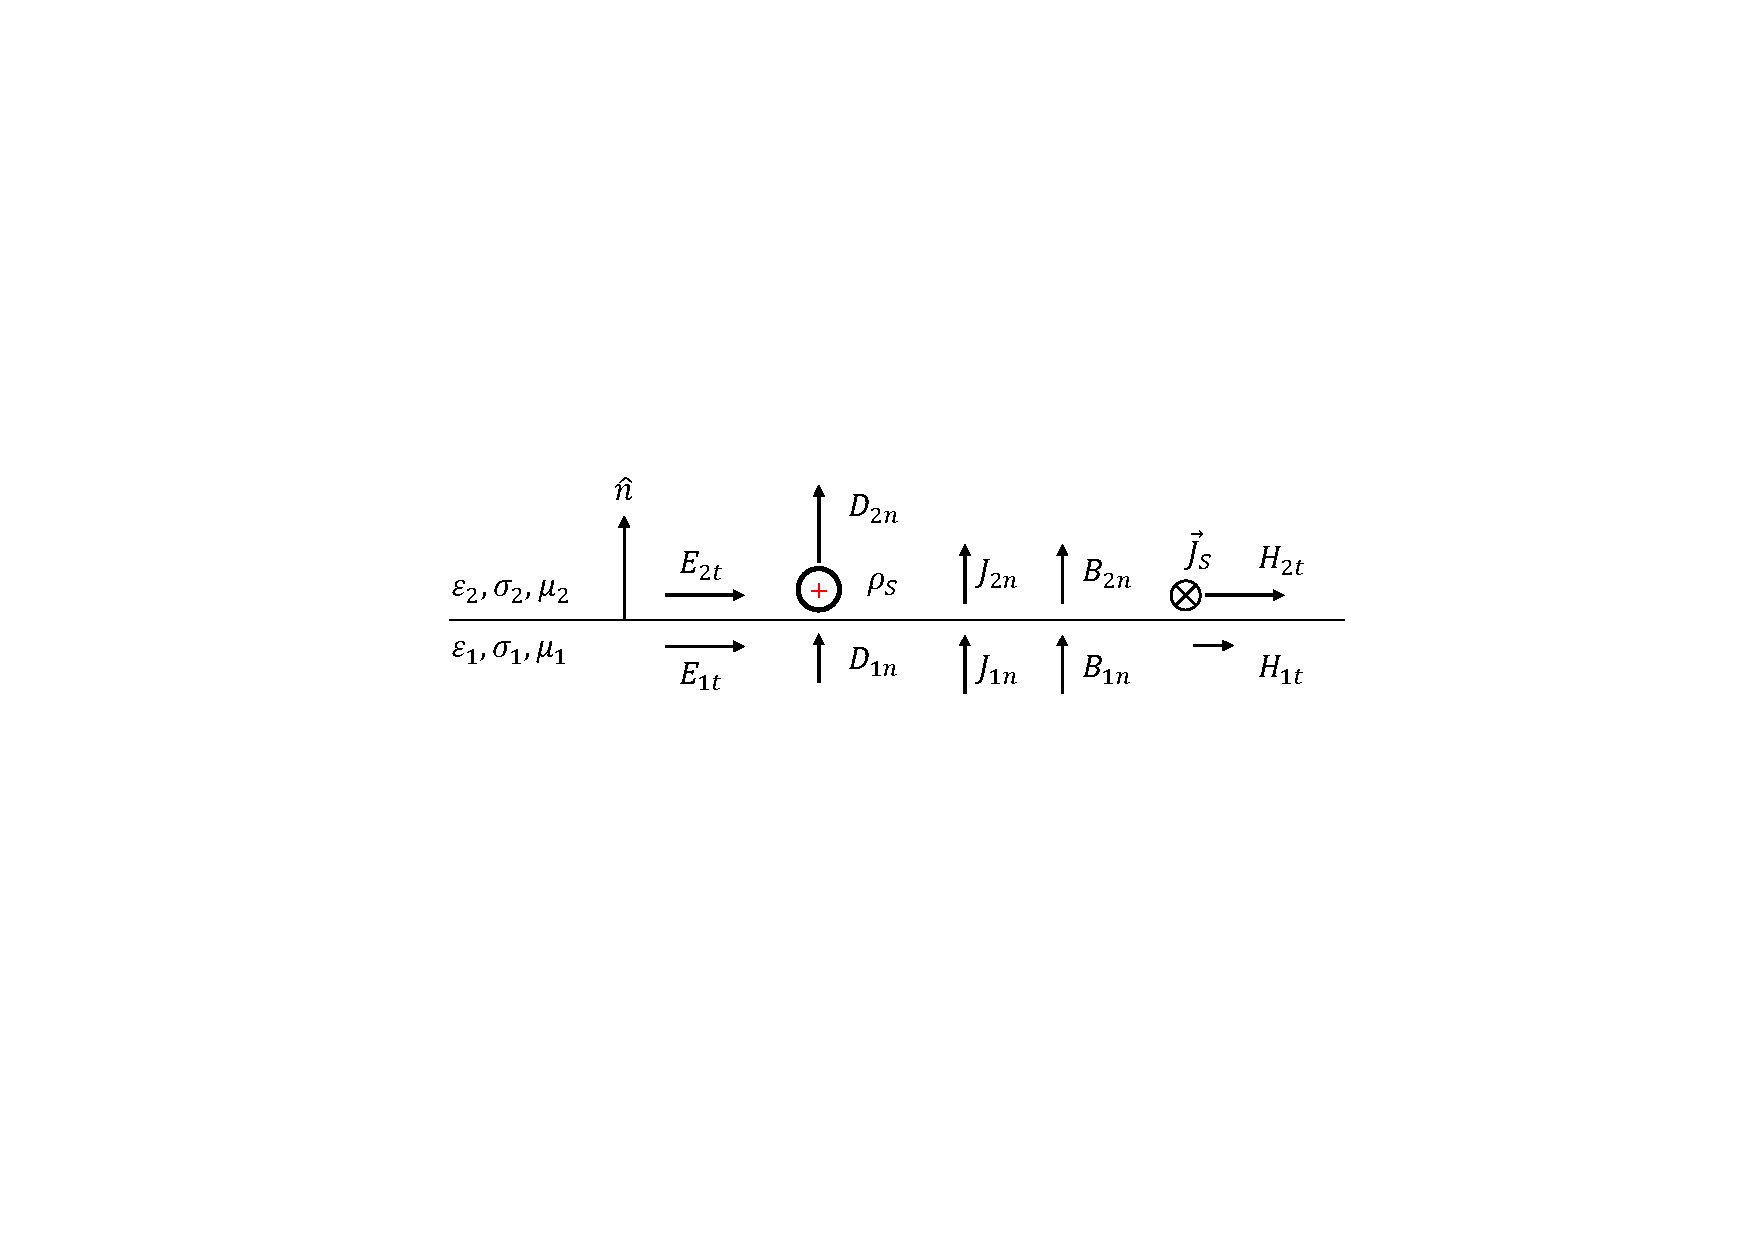
\includegraphics[width=10cm]{figure/5-1.pdf}
        \caption{\kaishu 一般介质界面边界条件示意图}\label{Fig: 介质边界条件示意图}
    \end{figure}

    特殊地,考虑两理想介质(1和2)的界面,以及理想导体(1)与理想介质(2)的界面处:
    \begin{subequations}
        \begin{numcases}{\mbox{理想介质1}\rightarrow\mbox{理想介质2}} 
            \hat{n}\cdot\left(\vec{D}_2-\vec{D}_1\right)=0\\
            \hat{n}\cdot\left(\vec{B}_2-\vec{B}_1\right)=0\\
            \hat{n}\times\left({\vec{E}}_2-{\vec{E}}_1\right)=0\\
            \hat{n}\times\left({\vec{H}}_2-{\vec{H}}_1\right)=0
        \end{numcases}
    \end{subequations}
    由此说明:两理想介质的界面处,电场、磁场沿任意方向连续;
    \begin{subequations}
        \begin{numcases}{\mbox{理想导体1}\rightarrow\mbox{理想介质2}} 
            \hat{n}\cdot\vec{D}_2=\rho_S\\
            \hat{n}\cdot\vec{B}_2=0\\
            \hat{n}\times{\vec{E}}_2=0\\
            \hat{n}\times{\vec{H}}_2=\vec{J}_S
        \end{numcases}
    \end{subequations}
    由此说明:PEC与理想介质的界面外部,电场垂直于界面,磁场平行于界面。


    \subsection{时谐电磁场的复矢量表示}
    {\color{gray}设正弦电场
    \begin{equation}
        \vec{E}=\vec{E}\left(x,y,z,t\right)=\left(E_x\left(x,y,z,t\right),E_y\left(x,y,z,t\right),E_z\left(x,y,z,t\right)\right)
    \end{equation}
    其每一个分量都是正弦量:
    \begin{equation}
        E_k\left(x,y,z,t\right)=E_{km}\left(x,y,z\right)\cos{\left(\omega t+\varphi_k\right)}
    \end{equation}
    其中$E_{km}$为空间一点的振幅在$\hat{k}$方向$(k=x,y,z)$上的分量,为实数。
    
    
    引入复振幅的好处在于,复振幅
    \begin{equation*}
        \dot{E}_{km}\left(x,y,z\right)=E_{km}\cdot \mathrm{e}^{\mathrm{j}(\omega t+\varphi_k)}
    \end{equation*}
    除了幅值外还可以表示电磁场的相位信息$\varphi_k$。由此,将原电场在$\hat{k}$方向上的分量作等量代换:
    \begin{equation}
        E_k\left(x,y,z\right)=\Re\left[{\dot{E}}_{km}\left(x,y,z\right)e^{\mathrm{j}\omega t}\right]
    \end{equation}
    原电场为
    \begin{equation}
        \vec{E}\left(x,y,z,t\right)=\Re\left[\left({\dot{E}}_{xm},{\dot{E}}_{ym},{\dot{E}}_{zm}\right)e^{\mathrm{j}\omega t}\right]
    \end{equation}
    又通常频率已经确定,省略掉$\cos{\omega t}$,则}定义电场强度的复矢量(in phasor form)为:
    \begin{equation}
        \dot{\vec{E}}(x,y,z)=\left({\dot{E}}_{xm},{\dot{E}}_{ym},{\dot{E}}_{zm}\right)
    \end{equation}
        其意义在于把时空的四维矢量函数简化成了空间的三维函数。


    复矢量表示下, 无源区域($\vec{J}=\vec{0},\,\rho=0$)  的麦克斯韦方程组变为:
    % \begin{subequations}
    %     \begin{numcases}{\mbox{}} 
    %         \nabla\times \dot{\bm{H}}=\mathrm{j}\omega \dot{\bm{D}} \\
    %         \nabla\times \dot{\bm{E}}=-\mathrm{j}\omega \dot{\bm{B}} \\
    %         \nabla\cdot \dot{\bm{B}}=0\\            
    %         \nabla\cdot \dot{\bm{D}}=0
    %     \end{numcases}
    % \end{subequations}
    
    \begin{subequations}
        \begin{align}
            &\nabla\times \dot{\vec{H}}=\mathrm{j}\omega \dot{\vec{D}} \\
            &\nabla\times \dot{\vec{E}}=-\mathrm{j}\omega \dot{\vec{B}} \\
            &\nabla\cdot \dot{\vec{B}}=0\\            
            &\nabla\cdot \dot{\vec{D}}=0
        \end{align}
    \end{subequations}


    \subsection{坡印廷定理}
    坡印亭(\emph{Pointing})定理:单位时间内输入一个闭合区域的的电磁能量,等于单位时间内区域内电场能量的增量,加上单位时间内区域的焦耳热。
    \begin{equation}
        -\oint_S\left(\vec{E}\times \vec{H}\right)\cdot \mathrm{d}\vec{S}
        =\frac{\partial }{\partial t}\int_V (\frac{1}{2}\vec{D}\cdot \vec{E}+\frac{1}{2}\vec{B}\cdot \vec{H})\,\mathrm{d}V
        +\int_V \vec{J}\cdot \vec{E}\,\mathrm{d}V
    \end{equation}

    定义坡印廷矢量$\vec{S}$(单位:\si{\watt\per\square\metre}):
    \begin{equation}
        \vec{S}=\vec{E}\times\vec{H}
    \end{equation}
    表示{\color{red}单位时间通过垂直单位面积的电磁能量},又称为{\color{red}电磁功率通量密度}。

    \vspace{5pt}
    \noindent\begin{boxedminipage}{\textwidth}
        \vspace{3pt}\setlength{\parindent}{2\ccwd}
        注意:$\oint_S \vec{S} \cdot \mathrm{d}\vec{S}$表示流出封闭曲面的总能流(单位:\si{\joule\per\second},也叫功率流,“流(flux)”强调该功率具有能速$\vec{v}_e=\frac{{\vec{S}}_{av}}{w_{av}}$),不能认为坡印廷矢量就代表电磁功率流密度。真正{\color{red}表示空间内一点功率流密度的是$\nabla\cdot \vec{S}$ } 而非$\vec{S}$本身。
        
        % {\color{gray}
        根据高斯定理有
        \begin{equation}
            \oint_S \vec{S} \cdot \mathrm{d}\vec{S}=\int_V \nabla\cdot \vec{S}\,\mathrm{d}V
        \end{equation}
        % }
        没有功率流动,说明无论闭合区域取多小,上积分式恒为0,即$\nabla·S=0$。说明这种情况下$\vec{S}$是一个旋度场,但并不一定有$\vec{S}=\vec{0}$。


        具体而言,在时变电磁场中,$\vec{S}$的物理意义表示电磁场的瞬时功率流密度,其曲面积分表示瞬时功率;但在静电场或静磁场中,$\vec{S}$并不代表功率流密度。
        {在静止的场中,没有功率的流动,能流密度不能代表功率的流动。}即虽然$\vec{S}\neq \vec{0}$但有$\nabla\cdot\vec{S}=0$
        \vspace{3pt}
    \end{boxedminipage}
    \vspace{5pt}


    定义平均坡印廷矢量(平均电磁功率通量密度):
    \begin{equation}
        {\vec{S}}_{av}=\frac{1}{T}\int_{0}^{T}{(\vec{E}\times\vec{H})\,\mathrm{d}t}=\frac{1}{2}\Re\left[\dot{\vec{E}}\times{\dot{\vec{H}}}^\ast\right]
    \end{equation}

    \subsection{波动方程}
    主要讨论均匀、线性,各向同性 介质的无源区域($\vec{J}=\vec{0},\,\rho=0$)内的情况。


    将介质的本构关系代入麦克斯韦方程组后,分别对第一、第二方程两边取旋度,利用矢量恒等式化简得:
    \begin{subequations}
        \begin{numcases}{\textbf{亥姆霍兹方程}} 
            \nabla^2  {\vec{E}}-\mu \varepsilon \frac{\partial^2  {\vec{E}}}{\partial t^2}=0 \\
            \nabla^2  {\vec{H}}-\mu \varepsilon \frac{\partial^2  {\vec{H}}}{\partial t^2}=0             
        \end{numcases}
    \end{subequations}
    可以将上式每个矢量方程分解为三个标量方程并求解,但这样很复杂。

    引入$\vec{E},\vec{H}$的复矢量,则 $\frac{\partial^2{\vec{E}}}{\partial t^2}=-\omega^2 \dot{\vec{E}}$,波动方程满足的偏微分方程变为:
    \begin{subequations}
        \begin{numcases}{\mbox{}} 
            \nabla^2\dot{\vec{E}}+ \omega^2 \mu \varepsilon \dot{\vec{E}}=0 \\
            \nabla^2\dot{\vec{H}}+ \omega^2 \mu \varepsilon \dot{\vec{H}}=0  
        \end{numcases}
    \end{subequations}
    并定义空间波数
    \begin{equation}
        k=\omega\sqrt{\mu \varepsilon}
    \end{equation}


\section{势函数及其解(矢位法)}
    通过求解辅助函数以得到电磁场,因此也称为辅助函数法。在微波/天线技术中,常用的辅助函数是\underline{矢量磁位}和\underline{标量电位},简称矢位和标位。

    \subsection{势函数及其规范}
    经典电动力学\footnote{不考虑Aharonov-Bohm效应(A-B效应),即认为磁场的物理效应可以完全用磁感应强度$\vec{B}$来描述,磁矢势$\vec{A}$不具有可观测的效应;也不考虑量子电动力学}所关心的是电荷的运动,而场作为一种物质其本身就是由它对其内电荷运动所产生的影响来刻画的(可以证明,验电荷在电磁场中的动能只与电荷量$e$,速度$\vec{v}$,以及电场磁场强度有关)。因此,如果两个电磁场能用同一组矢量$\vec{E}$和$\vec{B}$来表示,那么这两个场在物理上是全同的。
    % 电场和磁场是有物理意义的量,引入势函数仅仅是为了利于证明和计算。

    电场强度$\vec{E}$和磁感应强度$\vec{B}$只包含物理的自由度,即电磁场构型的每个自由度都对附近的验电荷的运动有单独可测量的效应。它们是关于势函数的单值函数:
    \begin{subequations}
        \begin{numcases}{\mbox{}} 
            \vec{E}=-\nabla \varphi-\frac{\partial \vec{A}}{\partial t}\\
            \vec{B}=\nabla\times\vec{A}
        \end{numcases}
    \end{subequations}
    
    但势函数除了包含物理自由度,还具有规范自由度,这是因为对于如下\textbf{势变换}:
    \begin{subequations}\label{Equ: 势变换}
        \begin{numcases}{\mbox{}} 
            \vec{A}\mapsto \vec{A}+\nabla \psi \\
            \varphi\mapsto \varphi-\frac{\partial \psi}{\partial t}
        \end{numcases}
        % \qquad $\psi(x,y,z;t)$为标量函数
    \end{subequations}

    电磁场的构型不变。即不同的势函数可以对应相同的电磁场。

    只有那些对于势变换\eqref{Equ: 势变换} 保持不变的量才有物理意义;特别是,所有方程在这个变换下必须是不变的。这种不变性称为\textbf{规范不变性}(德文为Eichinvarianz,英文为Gauge invariance)。


    因为势缺乏唯一性,我们就有可能去选择它们(即规范化:Guage fix),使它们满足我们所选择的附加条件。须指出,\underline{我们仅够令它们额外地满足一个标量等式}\footnote{这也解释了为什么库仑规范和洛伦兹规范只对磁矢势$\vec{A}$做出规定。因为引入一个关于$\vec{A}$的散度的标量方程后,$\varphi$也随之确定了},这是因为我们可以任意选择\eqref{Equ: 势变换}中的函数$\psi$。例如我们总可以选取合适的$\psi$,使得$\varphi=0$,即 Weyl gauge 。(但对于一个任意的$\vec{A}$,我们无法找到合适的$\psi$,使$\vec{A}=0$,因为这相当于引入了三个额外的条件。)除此之外还有 multipolar gauge,Fock Schwinger gauge, $R_\xi$ gauge 等等。

    其中常用的规范有库仑(Coulomb)规范和洛仑兹\footnote{是丹麦人ludvig Lorenz (1829—1891),在1867年提出了洛伦兹规范,并在前人基础上建立完善了滞后势:纽曼1845年在线圈互感的问题中提出了矢量势,黎曼可能在1857年左右得到了滞后势的概念,但是黎曼不幸去世,他的论文直到洛伦兹论文发表以后才出现。另一个洛伦兹是荷兰人Hendrik Lorentz (1853—1928),提出了相对论的洛伦兹变换。}(Lorenz)规范。

    \paragraph{库仑规范:}
    \begin{equation}
        \nabla\cdot\vec{A}=0
    \end{equation}
    库仑规范的优点是将麦克斯韦方程组关于电场的方程简化为静电场的形式:
    \begin{subequations}
        \begin{numcases}{\mbox{}} 
            \nabla^2 \varphi=-\frac{\rho}{\varepsilon}\label{Equ: 库仑规范下的第四方程}\\
            \nabla^2 \vec{A}=-\mu \vec{J}-\mu \varepsilon \frac{\partial \vec{E}}{\partial t}\label{Equ: 库仑规范下的第一方程}
        \end{numcases}
    \end{subequations}
        % 可以利用延迟格林函数,推迟势balabala,算出辐射的情况。

    {\color{gray}\begin{proof}
        将势函数与电场磁场的关系分别代入 第四方程 和 第一方程:
        \begin{equation*}
            \nabla\cdot\vec{E}
            =-\nabla^2 \varphi-\frac{\partial \left(\nabla\cdot\vec{A}\right)}{\partial t}
            =-\nabla^2 \varphi
            =\rho /\varepsilon
        \end{equation*}
        
        \begin{equation*}
            \nabla\times\vec{B}
            =\nabla\times \nabla\times\vec{A}=-\nabla^2 \vec{A}+\nabla \nabla\cdot\vec{A}
            =-\nabla^2 \vec{A}
            =\mu \left(\vec{J}+\frac{\partial \vec{D}}{\partial t}\right)
        \end{equation*}
    \end{proof}}

    得到的方程组中,电标位很好求:\hyperref[Equ: 库仑规范下的第四方程]{式(\ref*{Equ: 库仑规范下的第四方程})}正是静电场的泊松方程,它的解为:
    \begin{equation}
        \varphi(\vec{r},t)=\frac{1}{4\pi \varepsilon}\int\limits_V \frac{\rho(\vec{r}',t)}{|\vec{r}-\vec{r}'|}\,\mathrm{d}V'+\mathrm{const}
    \end{equation}
    这是体分布的电荷在场点$\vec{r}$处的电位,为了方便常取$\mathrm{const}=0$。若为面电荷或线电荷,则改变积分区域和微分单元即可。

    但是磁矢位满足的方程\eqref{Equ: 库仑规范下的第一方程},麦克斯韦自己也没有办法求解,只能考虑没有位移电流的特殊情况。所以麦克斯韦从来没有得到过像洛伦兹那样的滞后势解(即\hyperref[Equ: 滞后势的解]{式(\ref*{Equ: 滞后势的解})})。

    在无位移电流的情况(静电场)下,磁矢位满足的方程\eqref{Equ: 库仑规范下的第一方程}变为
    \begin{equation}
        \nabla^2 \vec{A}=-\mu \vec{J}
    \end{equation}
    只需类比泊松方程的解,得到
    \begin{equation}
        \vec{A}(\vec{r},t)=\frac{\mu}{4\pi}\int\limits_V \frac{\vec{J}(\vec{r}',t)}{|\vec{r}-\vec{r}'|}\,\mathrm{d}V'
    \end{equation}

    由此可见,库仑规范下认为电荷分布产生了势$\varphi$,电流分布产生了磁矢势$\vec{A}$,因果关系明了,且具有瞬态性(instantaneous)。
    
    缺点除了磁矢势不方便求解,还有不满足洛伦兹协变性(Lorentz invariance),在和狭义相对论结合的时候会出问题。
    
    \paragraph{洛伦兹规范}
    \begin{equation}
        \nabla\cdot\vec{A}+\mu \varepsilon\frac{\partial \varphi}{\partial t}=0
    \end{equation}
    % \begin{equation}
    %     \nabla\cdot\vec{A}+\frac{1}{c^2}\frac{\partial \varphi}{\partial t}=0
    % \end{equation}
    
    利用洛伦兹规范,则可以通过麦克斯韦方程组求解出势函数,过程如下:
    
    用辅助矢位和标位函数表示待求场矢量:
    \begin{subequations}
        \begin{numcases}{\mbox{}} 
            \vec{E}=-\nabla \varphi-\frac{\partial \vec{A}}{\partial t}\label{Equ: 辅助函数表示电场} \\
            \vec{H}=\frac{1}{\mu}\left(\nabla\times\vec{A}\right)
        \end{numcases}
    \end{subequations}
    代入第一方程,得:
    \begin{equation}
        \nabla\times \frac{1}{\mu}\nabla\times\vec{A}=\vec{J}+\varepsilon \frac{\partial }{\partial t}\left(-\nabla \varphi-\frac{\partial \vec{A}}{\partial t}\right)
    \end{equation}
    再将洛伦兹规范代入上式,化简得:
    \begin{subequations}\label{Equ: 辅助函数的达朗贝尔方程}
    \begin{equation}\label{Equ: 辅助函数的达朗贝尔方程A}
        \nabla^2 \vec{A}-\mu \varepsilon \frac{\partial^2 \vec{A}}{\partial t^2}=-\mu \vec{J}
    \end{equation}
    同理,将\hyperref[Equ: 辅助函数表示电场]{式(\ref*{Equ: 辅助函数表示电场})}和洛仑兹规范代入第四方程,可以得:
    \begin{equation}\label{Equ: 辅助函数的达朗贝尔方程phi}
        \nabla^2 \varphi-\mu \varepsilon \frac{\partial^2 \varphi}{\partial t^2}=-\frac{\rho}{\varepsilon}
    \end{equation}
    \end{subequations}
    \hyperref[Equ: 辅助函数的达朗贝尔方程A]{式(\ref*{Equ: 辅助函数的达朗贝尔方程A})}和\hyperref[Equ: 辅助函数的达朗贝尔方程phi]{式(\ref*{Equ: 辅助函数的达朗贝尔方程phi})}的形式相同,这种形式的波动方程称为\textbf{达朗贝尔方程}。

    达朗贝尔方程的标量形式可用格林定理求解,其解为:
    \begin{subequations}\label{Equ: 滞后势的解}
        \begin{numcases}{\mbox{}} 
            \vec{A}(\vec{r},t)=\frac{\mu}{4\pi}\int\limits_V \frac{\vec{J}(\vec{r}',t)\mathrm{e}^{-\mathrm{j}k|\vec{r}-\vec{r}'|}}{|\vec{r}-\vec{r}'|}\,\mathrm{d}V'\\
            \varphi(\vec{r},t)=\frac{1}{4\pi \varepsilon}\int\limits_V \frac{\rho(\vec{r}',t)\mathrm{e}^{-\mathrm{j}k|\vec{r}-\vec{r}'|}}{|\vec{r}-\vec{r}'|}\,\mathrm{d}V'
        \end{numcases}
    \end{subequations}

    \paragraph{规范化的实质和意义}
    ~\\ \vspace{-5pt}% 首先应指出,只有在经典动力学中,规范化才是不唯一的。
    
    满足势变换\eqref{Equ: 势变换}的两组不同的势函数其实对应同一个物理体系:它们是同一个电磁场的不同解。解不同的本质原因在于参照系不同。设想有一个理想的圆柱,如果被扭了但又保持圆柱的形状,你当然无法知道是否发生扭曲了。但是,若在圆柱的底端到顶端加一条曲线,则从曲线的变化可以判断是否发生了扭曲。这个过程就是一个 gauge fixing 的过程。规范化其说是添加约束,更准确地说是添加参照。注意,这条曲线是从外部加上去的,不属于考察的对象,因此也不应该影响考察对象的性质。

    {\color{gray}
        从数学的角度上,由于已经满足$\nabla\times\vec{A}=\vec{B}$,那么根据亥姆霍兹定理,唯一确定场矢量$\vec{A}$只需要再确定$\vec{A}$的散度即可。因此规范化的目的是为了求得唯一的磁矢势$A$。但是这种看法似乎认为是先给出$\vec{B}$,再求$\vec{A}$,而实际上物理学观点认为是先有磁矢势,再有磁场强度。
    }

    在求解经典电动力学的问题时,可以因具体问题的的方便程度人为选取一个gauge fix,选取得适当则可以使问题大大简化。


    \subsection{滞后势的求解}
    滞后势,即引入了矢量位和标量位来描述电磁场后,\underline{洛伦兹规范}下求得的磁矢势$\vec{A}$和电势$\varphi$。“滞后”体现在从源点$\vec{r}'$作用到场点$\vec{r}$,需要延迟$\frac{|\vec{r}-\vec{r}'|}{v}$的时间。换句话说,场点位函数的变化始终滞后于场源的变化,滞后的时间就是电磁波传播距离$R=|\vec{r}-\vec{r}'|$所需要的时间。(这与库伦规范下的势函数解具有瞬时性恰好矛盾)

    \begin{lemma}[格林定理]
        $u,w$为任意标量函数,且$u,w$以及它们的一阶、二阶导数在$V$内连续,则
        \begin{equation}
            \int\limits_V (u \nabla^2w-w \nabla^2u)\,\mathrm{d}V=\oint\limits_S (u \nabla w-w \nabla u)\cdot\mathrm{d}\vec{S}
        \end{equation}
    \end{lemma}

    令其中$u=\varphi,\;w=\psi=\frac{\mathrm{e}^{-\mathrm{j}k R}}{R}$,则在$V$内除$R=0\,(\vec{r}'=\vec{r})$外的区域,$\psi$符合格林定理中标量函数的约束条件。不妨假设$\varphi$也在该区域内符合条件。

    为了排除被积函数的奇点(不让积分变点$\vec{ r}'$取到场点$\vec{r}$),则以场点$\vec{r}$为圆心,作一半径为$a$的小球,其表面为$S_2$,体积为$V_2$。于是积分体积变为$V_1=V-V_2$,积分表面变为$S_1=S+S_2$。

    由格林定理:
    \begin{equation}\label{Equ: 方程求解滞后势}
        \int\limits_{V_1}\left[\varphi \nabla^2\psi-\psi \nabla^2 \varphi\right]\,\mathrm{d}V'
        =\oint\limits_{S} \left[\varphi \frac{\partial \psi}{\partial \hat{n}}-\psi \frac{\partial \varphi}{\partial \hat{n}}\right]\cdot\mathrm{d}\vec{S}'
        +\oint\limits_{S_2} \left[\varphi \frac{\partial \psi}{\partial \hat{n}}-\psi \frac{\partial \varphi}{\partial \hat{n}}\right]\cdot\mathrm{d}\vec{S}'
    \end{equation}
    这里用到了恒等式
    \begin{equation*}
        \nabla \varphi \cdot \hat{n}\mathrm{d}S
        =\left(\frac{\partial \varphi}{\partial x}\hat{x}+\frac{\partial \varphi}{\partial y}\hat{y}+\frac{\partial \varphi}{\partial z}\hat{z}\right)\cdot \mathrm{d}\vec{S}
        =\frac{\partial \varphi}{\partial \hat{n}}\cdot \mathrm{d}\vec{S}
        =\frac{\partial \varphi}{\partial n}\mathrm{d}S
    \end{equation*}
    其中$\frac{\partial \varphi}{\partial n}$即$\varphi$沿$\hat{n}$方向的方向导数,也等于此处电场沿$\hat{n}$方向的分量的相反数。

    注意到,积分变点$\vec{r}'\in S_2$时,$\hat{n}$($\mathrm{d}\vec{S}$)恒指向小球球心,其方向与变量$R$增大的方向相反,因此$\frac{\partial \;\cdot }{\partial n}=-\frac{\partial \;\cdot}{\partial R}$。
    
    且有立体角元定义
    \begin{equation}
        \mathrm{d}\varOmega=\frac{\mathrm{d}A}{r^2}=\sin\theta \,\mathrm{d}\theta \,\mathrm{d}\phi
    \end{equation}
    
    因此
    \begin{equation*}
        \begin{aligned}
            \oint\limits_{S_2} \left[\varphi \frac{\partial \psi}{\partial \hat{n}}-\psi \frac{\partial \varphi}{\partial \hat{n}}\right]\cdot\mathrm{d}\vec{S}'
            &=\oint\limits_{S_2} \left[-\varphi \frac{\partial \psi}{\partial R}+\psi \frac{\partial \varphi}{\partial R}\right]_{R=a} \,a^2\mathrm{d}\varOmega'\\
            &=\oint\limits_{S_2} \left[-\varphi \left(-\frac{1}{R^2}-\frac{\mathrm{j}k}{R}\right)\mathrm{e}^{-\mathrm{j}k R}+ \frac{\mathrm{e}^{-\mathrm{j}kR}}{R} \frac{\partial \varphi}{\partial R}\right]_{R=a} \,a^2\mathrm{d}\varOmega'\\
            &=\oint\limits_{S_2} \left[\left.\varphi(\vec{r}')\right\vert_{R=a} \left(1+\mathrm{j}ka\right)\mathrm{e}^{-\mathrm{j}ka}+ a\mathrm{e}^{-\mathrm{j}ka}\left.\frac{\partial \varphi}{\partial R}\right\vert_{R=a}\right] \,\mathrm{d}\varOmega'
        \end{aligned}
    \end{equation*}

    由于$\varphi, \frac{\partial \varphi}{\partial R}$均有限,上式在$a\rightarrow 0$时将收敛于:
    \begin{equation*}
        \lim_{a \to 0}{\oint\limits_{S_2} \left[\varphi \frac{\partial \psi}{\partial \hat{n}}-\psi \frac{\partial \varphi}{\partial \hat{n}}\right]\cdot\mathrm{d}\vec{S}'}
        =\lim_{a \to 0}{\oint\limits_{S_2}\left.\varphi(\vec{r}')\right\vert_{R=a}\,\mathrm{d}\varOmega'}
        =\varphi(\vec{r})\oint\limits_{S_2}\,\mathrm{d}\varOmega'
        =4\pi\varphi(\vec{r})
    \end{equation*}
    后两个等号成立是因为,小球无限缩小时$\left.\varphi(\vec{r}')\right\vert_{R=a}$可用球心处的电势$\varphi(\vec{r})$代替,且所有封闭曲面内的立体角元积分均为$\int_{0}^{\pi}\int_{0}^{2\pi}\sin\theta \,\mathrm{d}\theta \,\mathrm{d}\phi=4\pi$。

    将上式极限$a\rightarrow 0$时的结论代入到方程(\eqref{Equ: 方程求解滞后势})中,得:
    \begin{equation}
        \begin{aligned}
            \varphi(\vec{r})
            &=\frac{1}{4\pi}\lim_{a \to 0}\left\{\int\limits_{V_1}\left[\varphi \nabla^2\psi-\psi \nabla^2 \varphi\right]\,\mathrm{d}V'
            -\oint\limits_{S} \left[\varphi \frac{\partial \psi}{\partial \hat{n}}-\psi \frac{\partial \varphi}{\partial \hat{n}}\right]\cdot\mathrm{d}\vec{S}'\right\}\\
            &=\frac{1}{4\pi}\left\{\int\limits_{V}\left[\varphi \nabla^2\psi-\psi \nabla^2 \varphi\right]\,\mathrm{d}V'
            -\oint\limits_{S} \left[\varphi \frac{\partial \psi}{\partial \hat{n}}-\psi \frac{\partial \varphi}{\partial \hat{n}}\right]\cdot\mathrm{d}\vec{S}'\right\}\\
        \end{aligned}
    \end{equation}

    注意到在时谐场的条件下,$\varphi$和$\psi$都满足亥姆霍兹方程:
    \begin{subequations}
        \begin{numcases}{\mbox{}} 
            \nabla^2\psi+k^2\psi=0\\
            \nabla^2 \varphi+k^2 \varphi=-\frac{\rho}{\varepsilon}
        \end{numcases}
    \end{subequations}

    将$\nabla^2 \varphi$和$\nabla^2\psi$代入化简,得:
    \begin{equation}\label{Equ: 亥姆霍兹积分}
        \begin{aligned}
            \varphi(\vec{r})
            &=\frac{1}{4\pi}\left\{\int\limits_{V}\psi \frac{\rho(\vec{r}')}{\varepsilon}\,\mathrm{d}V'
            -\oint\limits_{S} \left[\varphi \frac{\partial \psi}{\partial n}-\psi \frac{\partial \varphi}{\partial n}\right]\,\mathrm{d}S'\right\}\\
            &=\frac{1}{4\pi \varepsilon}\int\limits_{V}\psi \rho(\vec{r}')\,\mathrm{d}V'
            -\frac{1}{4\pi}\oint\limits_{S} \left[\varphi \frac{\partial \psi}{\partial n}-\psi \frac{\partial \varphi}{\partial n}\right]\,\mathrm{d}S' % \\
            % &=\frac{1}{4\pi \varepsilon}\int\limits_{V}\frac{\rho(\vec{r}')\mathrm{e}^{-\mathrm{j}kR}}{R}\,\mathrm{d}V'
            % -\frac{1}{4\pi}\oint\limits_{S} \left[\varphi(\vec{r}') \frac{\partial}{\partial n}\left(\frac{\mathrm{e}^{-\mathrm{j}kR}}{R}\right)-\frac{\partial \varphi(\vec{r}')}{\partial n}\frac{\mathrm{e}^{-\mathrm{j}kR}}{R}\right]\,\mathrm{d}S'
        \end{aligned}
    \end{equation}

    同理构造标量函数$\psi$结合格林定理,可以解出磁矢势。至此,我们已经求解出了洛伦兹规范下满足时谐场条件的滞后势:
    \begin{subequations}\label{Equ: 滞后势的初始解}
        \begin{numcases}{\mbox{}} 
            \varphi(\vec{r})
            =\frac{1}{4\pi \varepsilon}\int\limits_{V}\frac{\rho(\vec{r}')\mathrm{e}^{-\mathrm{j}kR}}{R}\,\mathrm{d}V'
            -\frac{1}{4\pi}\oint\limits_{S} \left[\varphi(\vec{r}') \frac{\partial}{\partial n}\left(\frac{\mathrm{e}^{-\mathrm{j}kR}}{R}\right)-\frac{\partial \varphi(\vec{r}')}{\partial n}\frac{\mathrm{e}^{-\mathrm{j}kR}}{R}\right]\,\mathrm{d}S'\\
            \vec{A}(\vec{r})
            =\frac{\mu}{4\pi}\int\limits_{V}\frac{\vec{J}(\vec{r}')\mathrm{e}^{-\mathrm{j}kR}}{R}\,\mathrm{d}V'
            -\frac{1}{4\pi}\oint\limits_{S} \left[\vec{A}(\vec{r}') \frac{\partial}{\partial n}\left(\frac{\mathrm{e}^{-\mathrm{j}kR}}{R}\right)-\frac{\partial \vec{A}(\vec{r}')}{\partial n}\frac{\mathrm{e}^{-\mathrm{j}kR}}{R}\right]\,\mathrm{d}S'
        \end{numcases}
    \end{subequations}
    该结论首先由亥姆霍兹得出,故称形如\hyperref[Equ: 亥姆霍兹积分]{式(\ref*{Equ: 亥姆霍兹积分})}的积分式为亥姆霍兹积分。

    结果表明,空间中的滞后势由两部分场源贡献:体积分的部分表示体积$V$内的源,闭合面$S$上的积分表示$V$外场源的贡献。

    \subsection{辐射条件}
    在考虑无限空间中的电磁问题时,设积分曲面$S$为半径$R$的球面。由于\hyperref[Equ: 滞后势的初始解]{式(\ref*{Equ: 滞后势的初始解})}中面积分的单位矢量$\hat{n}$指向$R$增大的方向,有$\frac{\partial \;\cdot}{\partial n}=\frac{\partial \;\cdot}{\partial R}$,可以将面积分写为:
    \begin{equation*}
        -\frac{1}{4\pi} \oint\limits_S \left[\varphi(\vec{r}')\left(-\frac{1}{R^2}-\frac{\mathrm{j}k}{R}\right)\mathrm{e}^{-\mathrm{j}k R} - \frac{\partial \varphi(\vec{r}')}{\partial R} \frac{\mathrm{e}^{-\mathrm{j}kR}}{R}\right] \mathrm{d}S'
    \end{equation*}
    再使用立体角代换$\mathrm{d}S'=R^2 \mathrm{d}\varOmega'$,面积分等价于:
    \begin{equation}
        \frac{1}{4\pi} \oint\limits_S \left[\varphi(\vec{r}')\left(1+\mathrm{j}kR\right)\mathrm{e}^{-\mathrm{j}k R} + R\frac{\partial \varphi(\vec{r}')}{\partial R} \mathrm{e}^{-\mathrm{j}kR}\right] \mathrm{d}\varOmega'
    \end{equation}

    为了排除无限远处的场源,就要使无限远处场源的积分贡献为0,也就是要使上式面积分为0结果。
    
    则得到辐射条件:
    \begin{subequations}
        \begin{numcases}{} 
            \mbox{电标位的辐射条件:}\lim_{R \to \infty}{R\left(\frac{\partial \varphi(\vec{r}')}{\partial R}+\mathrm{j}k \varphi(\vec{r}')\right)}=0\\
            \mbox{磁矢位的辐射条件:}\lim_{R \to \infty}{R\left(\frac{\partial \vec{A}(\vec{r}')}{\partial R}+\mathrm{j}k \vec{A}(\vec{r}')\right)}=0
        \end{numcases}
    \end{subequations}

    辐射条件的本质是:要求 \underline{场源产生的滞后势在远离场源的空间中至少要以$R^{-1}$的速度衰减}。

    满足辐射条件的滞后势简化为:
    \begin{subequations}\label{Equ: 辐射场的滞后势解}
        \begin{numcases}{\mbox{}} 
            \varphi(\vec{r})
            =\frac{1}{4\pi \varepsilon}\int\limits_{V}\frac{\rho(\vec{r}')\mathrm{e}^{-\mathrm{j}kR}}{R}\,\mathrm{d}V'\\
            \vec{A}(\vec{r})
            =\frac{\mu}{4\pi}\int\limits_{V}\frac{\vec{J}(\vec{r}')\mathrm{e}^{-\mathrm{j}kR}}{R}\,\mathrm{d}V'
        \end{numcases}
    \end{subequations}

\section{电基本振子}

    电基本振子是一段载有高频电流的线元。其长度$\Delta  l\ll \lambda$,故认为其上各点电流振幅相同,相位相同。

    \subsection{电基本振子的辐射场}
    设电流元沿$\hat{z}$方向。根据辐射条件下的磁矢位解,有
    \begin{equation}
        \begin{aligned}
            \vec{A}(\vec{r})&=\frac{\mu}{4\pi}\int\limits_{V}\frac{\vec{J}(\vec{r}')\mathrm{e}^{-\mathrm{j}kR}}{R}\,\mathrm{d}V'\\
            &=\frac{\mu}{4\pi}\int\limits_{l}\frac{I\hat{z}}{\Delta S}\frac{\mathrm{e}^{-\mathrm{j}kR}}{R}\,\Delta S\mathrm{d}l'\\
            &=\frac{\mu}{4\pi}\frac{\mathrm{e}^{-\mathrm{j}kr}}{r}\int\limits_{l}I\hat{z}\,\mathrm{d}l'\qquad\mbox{\color{gray}$(\Delta l\ll R)$}\\
            &=\frac{\mu I \Delta l}{4\pi r}\mathrm{e}^{-\mathrm{j}kr}\hat{z}
        \end{aligned}
    \end{equation}
    注意,当$\vec{J}(\vec{r}')$为复矢量时,$I$为复数(电流相量):$\dot{I}=\dot{I}_m \mathrm{e}^{\mathrm{j}\varphi_{I0}}=I_m\cos(\omega t+\varphi_{I0})$省略上标$\dot{~}$的形式。

    使用相量表示电压电流,则
    \begin{equation}
        Q=\frac{I}{\mathrm{j}\omega}
    \end{equation}
    表示电流元两端聚积的大小相等,符号相反的时谐电荷量。

    {\color{gray} 由此可以求得标量电位
    \begin{equation}
        \begin{aligned}
            \varphi(\vec{r})
            &=\frac{1}{4\pi \varepsilon}\int\limits_{V}\frac{\rho(\vec{r}')\mathrm{e}^{-\mathrm{j}kR}}{R}\,\mathrm{d}V'\\
            &=\frac{1}{4\pi \varepsilon}\int\limits_{l}\frac{\frac{Q}{\Delta S \mathrm{d}l}\mathrm{e}^{-\mathrm{j}kR}}{R}\, \Delta S\mathrm{d}l'\\
            &=\frac{Q}{4\pi \varepsilon r}\mathrm{e}^{-\mathrm{j}kr}
        \end{aligned}
    \end{equation}
    }

    引入球坐标系以便于研究电基本振子的辐射场:
    \begin{equation}
        \vec{A}=\hat{r}A_r+\hat{\theta}A_\theta+\hat{\phi}A_\phi=\hat{r}A_z\cos\theta-\hat{\theta}A_z\sin\theta
    \end{equation}
    其中$\hat{\theta}$前的负号是由于$\hat{z}A_z$在沿$\hat{r}$和$\hat{\theta}$正交分解时,$A_\theta$分量的方向与$\hat{\theta}$增大的方向相反。

    由$\vec{A}$表示磁场:
    \begin{equation}
        \begin{aligned}
            \vec{H}(\vec{r})=\frac{1}{\mu}\nabla\times \vec{A}
            =\frac{1}{\mu r^2\sin\theta}\begin{vmatrix}
                \hat{r}&r\hat{\theta}&r\sin\theta\hat{\phi}\\
                \frac{\partial }{\partial r}&\frac{\partial }{\partial \theta}&\frac{\partial }{\partial \phi}\\
                A_z\cos\theta&-rA_z\sin\theta&0
            \end{vmatrix}
        \end{aligned}
    \end{equation}

    再由麦克斯韦方程组第一方程,$\vec{E}=\frac{1}{\mathrm{j}\omega \varepsilon}\nabla\times \vec{H}$,可以解出辐射场:

    \begin{equation}
        \begin{array}{l c cc cc}
            \vec{H}=&\hat{r}0 &+&\hat{\theta}0&+&\hat{\phi}\frac{I \mathrm{d}l\sin\theta}{4\pi}\left[\frac{\mathrm{j}k}{r}+\frac{1}{r^2}\right]\mathrm{e}^{-\mathrm{j}k r}\\
            \vec{E}=&\hat{r}\frac{2I \mathrm{d}l\cos\theta}{4\pi \varepsilon \mathrm{j}\omega}\left[\frac{\mathrm{j}k}{r^2}+\frac{1}{r^3}\right]\mathrm{e}^{-\mathrm{j}k r} &+&\hat{\theta}\frac{I \mathrm{d}l\sin\theta}{4\pi \varepsilon \mathrm{j}\omega}\left[-\frac{k^2}{r}+\frac{\mathrm{j}k}{r^2}+\frac{1}{r^3}\right]\mathrm{e}^{-\mathrm{j}k r}&+&\hat{\phi}0\\
        \end{array}
    \end{equation}

    


\chapter{天线的电参数}
\begin{equation*}
\mbox{天线参数}
\begin{cases}
    \mbox{电路参量}
    \begin{cases}
        \mbox{天线阻抗}\\
        \mbox{辐射电阻}
    \end{cases}\\
    \mbox{空间参量}
    \begin{cases}
        \mbox{场波瓣图}\\
        \mbox{功率波瓣图}\\
        \mbox{定向性}D\\
        \mbox{增益}G\\
        \mbox{极化}\mathrm{LP},\mathrm{CP},\mathrm{EP}
    \end{cases}
\end{cases}
\end{equation*}

    \subsection{辐射方向图和对称振子方向图}
    \paragraph{辐射方向图}:天线的辐射特性是关于空间坐标的函数,若在固定距离上,此函数通过数学函数或者图形来描述,则得到的数学函数或者图形即为辐射方向图,简称方向图。

    注意:\begin{itemize}

        \item 辐射特性有功率通量密度(Power flux density)、辐射强度(Radiation intensity)、场强(Fields strength)、相位(Phase)、极化(Polarization)等;
        \item 空间坐标有三维坐标系或者二维坐标系;
        \item 固定距离:坐标原点到观察点的距离保持不变。根据远场条件,功率方向图和场强方向图与距离$r$无关,而相位方向图与距离有关。
        \item 三维方向图是一系列二维方向图的组合。通过几组方向图即可得到所需要的天线辐射性能信息。工程上用两个相互垂直的主平面内的方向图表示;
        \item 方向图一般描述天线远场区的辐射特性;
        \item 
    \end{itemize}
    
    方向图中主要关注的参数:
    \begin{enumerate}
        \item 零功率波瓣宽度(FNBW) $2\theta_{OE}$ 和 $2\theta_{OH}$:指主瓣最大值两边两个零辐射方向的夹角。
        \item 半功率波瓣宽度(HPBW) $2\theta_{OE}$ 和 $2\theta_{OE}$:指主瓣最大值两边功率通量密度下降到最大值的一半(或场强下降到最大值的0.707)时,即下降3dB的两点间的夹角。
        \item 旁瓣电平(FSLL):指第一旁瓣功率密度和主瓣功率密度之比的对数值:
            \begin{equation}
                \xi_1=10\lg\frac{S(\theta_1,\varphi_1)}{S} 
            \end{equation}
        副瓣方向通常是不需要辐射或接收能量的方向。因此,天线副瓣电平愈低,表明天线在不需要方向上辐射或接收的能量愈弱,或者说在这些方向上对杂散的来波抑制能力愈强,抗干扰能力就愈强。因此,在天线设计中常有低副瓣设计要求如基站的上旁瓣、雷达天线。
        ④前后向抑制比:后瓣最大辐射方向上功率密度和主瓣功率密度之比的对数值。
        S,
        5= 101g'm =201g
        (dB)
        s,
        
    \end{enumerate}


    \paragraph{场强方向图函数}

    \paragraph{归一化方向图函数}
    某天线的方向图为$f(\theta,\varphi)$,则归一化方向图为$F(\theta,\varphi)=f(\theta,\varphi)/f_\mathrm{max}$。具体地,设$S(\theta,\varphi)$和$E(\theta,\varphi)$为(0,p)的功率通量密度和电场强度,归一化功率方向图p(O,)和归一化场强方向图为:

    \subsection{对称振子的辐射场}
    求解将对称振子分为许多小段,则每一小段都可看做一电基本振子,对于线性媒质,应用叠加原理,则对称振子的辐射场就等于这些无数小段基本振子辐射场的叠加。
    对称振子的电流分布近似为

    式中α:振子电流的相移常数。
    如果不考虑振子电流由辐射引起的
    衰减,忽略振子粗细的影响

    \subsection{辐射功率和辐射电阻}
    天线的输入功率一般为复功率,根据玻印廷定理,取包围天线所在体积$V$的任意封闭面$S$
    \begin{equation}
        \dot{p}_A=p_l+\dot{p}_\Sigma
    \end{equation}

    $V$内的损耗功率(导体损耗和介质损耗)
    \begin{equation}
        p_l=
    \end{equation}
天线的全辐射功率
=R+j2
='Reg,(E×H')-d.
天线的辐射功率
f
辐射的无功功率
=士1m)手,(E×H )-ask
+j2o(Wm一WR)


    辐射功率与线天线上电流的大小有关,不便于直接比较天线的性能。为此引入天线的辐射阻抗概念。假设天线的全辐射功率被一个等效阻抗所“吸收”,该阻抗上流过的电流为天线上某处的电流,称此等效阻抗为天线的辐射阻抗。如天线上某处电流的振幅为I,则辐射阻抗
    \begin{equation}
        Z_\Sigma=\frac{P_\Sigma+\mathrm{j}Q_\Sigma}{\frac{1}{2}I^2}=R_\Sigma+\mathrm{j}X_\Sigma
    \end{equation}

    使用 波腹电流$I_M$ 或 输入电流$I_A$ 来计算,可以得到不同意义下的辐射阻抗$Z_\Sigma$和$Z_{\Sigma A}$,
    两种阻抗值不同,但满足
    
    \begin{equation}
        \frac{1}{2}=
    \end{equation}

    采用玻印廷矢量法计算天线的实辐射功率(以后简称辐射功率)和辐射电阻。

    \subsection{辐射功率和辐射阻抗}

    \begin{equation*}
    \mbox{计算辐射功率和辐射阻抗}
    \begin{cases}
        \mbox{远场区——Poynting矢量法,辐射实功率,辐射电阻}\\
        \mbox{近场区——感应电势法,复功率,辐射电阻和电抗}
    \end{cases}
    \end{equation*}

    远场区辐射功率
    \begin{equation}
        P_\Sigma=\frac{1}{120\pi}
    \end{equation}

    辐射电阻
    \begin{equation}
        R_\Sigma=\frac{2P_\Sigma}{|I_M|^2}=60 \int_{0}^{\pi}\frac{[]^2}{\sin\theta}\,\mathrm{d}\theta
    \end{equation}

    \subsection{天线的有效长度}
    \subsection{方向系数}
    天线的方向系数:用数字定量地表示辐射电磁能量集束程度,描述天线的方向特性数,又叫做方向性系数或方向性增益。

    \begin{definition}[辐射强度]
        天线在某方向的辐射强度是该方向每单位立体角内的辐射功率:
        \begin{equation}
            U(\theta,\varphi)=
        \end{equation}
    \end{definition}

    \begin{definition}[方向系数]
        天线在某方向的方向系数$D(\theta,\varphi)$是该刀回辐别独度$U(\theta,\varphi)$与平均辐射强度之比,平均辐射强度为$\frac{1}{4}$,即
        \begin{equation}
            D(\theta,\varphi)=\frac{4\pi F^2(\theta,\varphi)}{\int_{0}^{2\pi}\int_{0}^{\pi}F^2(\theta,\varphi)\sin\theta\,\mathrm{d}\theta\mathrm{d}\varphi}
        \end{equation}

        最大辐射方向的方向系数:某天线的方向系数通常均指最大辐射方向的方向系数。

    \end{definition}

    \begin{definition}[天线增益]
        天线的在某方向的增益$G(\theta,\varphi)$是该方向辐射强度$U(\theta,\varphi)$同天线 \underline{以同一输入功率} 向空间均匀辐射的辐射强度$\dfrac{P_A}{4\pi}$之比,即
        \begin{equation}
            G(\theta,\varphi)=4\pi \frac{U(\theta,\varphi)}{P_A}
        \end{equation}

        增益与方向系数的关系
        \begin{equation}
            G(\theta,\varphi)=D(\theta,\varphi)\eta_A
        \end{equation}

        某天线的增益通常指最大辐射方向增益:
        \begin{equation}
            G=4\pi \frac{U_M}{P_A}=D_M\eta_A
        \end{equation}
    \end{definition}
    \subsection{对称振子的输入阻抗}
    
\section{}

\chapter{缝隙天线和微带天线}

缝隙天线是在金属壁(同轴线、波导管、谐振器)上开窄缝($<\frac{1}{2}\lambda$)所形成的的天线。


    \paragraph{Lone等效原理}

\section{理想缝隙天线}

    \subsection{电磁场的巴俾涅原理和缝隙天线}
    
    \begin{theorem}[巴俾涅原理]
        巴俾涅原理用于论述互补平面屏(理想导电屏和理想导磁屏)的矢量电磁场问题。
    \end{theorem}

    \begin{corollary}[电屏和互补磁屏的互补原理]
        ddd    
    \end{corollary}

    电屏(b)与互补电屏(d)之间的电磁场关系:
    \begin{subequations}
        \begin{numcases}{\mbox{}} 
            \vec{E}_e+Z_0 \vec{H}_d=\vec{E}^i\\
            \vec{H}_e-Y_0 \vec{E}_d=\vec{H}^i            
        \end{numcases}
    \end{subequations}


    无限大平板上的$\frac{\lambda}{2}$缝隙天线和半波振子具有互补的场分布。方向图相同,只是E面和H面互换。


    缝隙天线的辐射磁场:
    \begin{equation}
        \vec{E}_d=\mathrm{j}\frac{120U_M}{Z_0}\frac{\cos(kl\cos\theta)-\cos(kl)}{\sin\theta} \frac{\mathrm{e}^{-\mathrm{j}k r}}{r} \hat{\varphi}
    \end{equation}

    若令$U_M=0.5 Z_0I_M$,则它们的辐射场相同,因而辐射功率也相同。类比对称振子天线把辐射功率归于波腹电流和辐射电阻,缝隙天线的辐射功率可归于波腹电压和辐射电导:
    \begin{equation}
        P_{\varSigma '}=\frac{1}{2}\left\vert U_M\right\vert^2G_{\varSigma '}
    \end{equation}


\section{矩形波导缝隙天线}
    
    
    \subsection{波导缝隙天线阵列}
    为了增强天线阵列的方向性,在波导上按一定规律开出一系列尺寸相同的缝隙,构成波导缝隙阵列(Slot Array)。

    \paragraph{谐振式缝隙阵}
    \begin{enumerate}
    \renewcommand*\labelenumi{\circled{\theenumi}}
        \item 横向
        \item 纵向
    \end{enumerate} 

    \paragraph{非谐振式缝隙阵}
    若把谐振式缝隙阵的波导的末端改为匹配负载(使波导传输行波),且缝隙的间距不等于$\frac{\lambda}{2}$,则可以构成非谐振式缝隙阵。

    \underline{因为非谐振式缝隙阵是由行波激励的 ,所以能在较宽的频带内保持良好匹配,缺点是效率较低。}
    由天线阵列的理论,这种线性相位差的阵元构成的缝隙阵列,方向图指向与缝隙面法线的夹角为
    \begin{equation}
        \theta_M=\arcsin\left(\frac{\beta \lambda}{2 \pi d}\right)
    \end{equation}
    其中$\beta=\frac{2 \pi d}{\lambda_g}$。


    \paragraph{匹配偏斜缝隙阵}
    在窄壁上开斜缝,相邻斜缝之间的距离为$\frac{\lambda}{2}$,




    \subsection{波导缝隙阵的方向性}
    设$N$为缝隙个数,$\theta$为场点指向与缝隙平面法线的夹角。若各缝隙为等幅激励,则在$z$轴与缝隙平面法线所在的平面内:
    \begin{equation}
        f_a(\theta)=f(\theta)\frac{\sin\left[\frac{N}{2}(kd\sin\theta-\beta)\right]}{\sin\left[\frac{1}{2}(kd\sin\theta-\beta)\right]}
    \end{equation}



\section{微带天线}

    \subsection{微带天线的结构}

    \subsection{微带天线的辐射原理}

    \subsection{微带天线的分析方法}
    将矩形微带的两个开路端等效为两个缝隙天线。


\section{常见宽带天线}

    \subsection{菱形天线}    
    
    \subsection{螺旋天线}
        
    \subsection{非频变天线}
    任何天线,它的性能都是由电尺寸(长度与波长的比值,或者面积与波长的平方的比值)决定的。

    如果天线的所有尺寸和工作波长按同比例变化,则天线的辐射性质保持不变。

    \begin{enumerate}
    \renewcommand*\labelenumi{\circled{\theenumi}}
        \item 角度条件。 天线的几何形状只由角度角度决定,与其他尺寸无关。
        \item 终端效应弱。 天线向外辐射的功率主要在传输线上消耗。决定天线辐射特性的主要部分是载有较大电流的部分,而其延伸段的作用很小,在这种情况下,有限长天线具有与无限长天线相似的电性能。
    \end{enumerate}

    平面等角螺旋天线的结构和工作原理
    \begin{subequations}
        \begin{numcases}{\mbox{双臂四线的极坐标方程}} 
            r_1=r_0 \mathrm{e}^{\alpha \varphi}\\
            r_2=r_0 \mathrm{e}^{\alpha (\varphi-\delta)}\\
            r_3=r_0 \mathrm{e}^{\alpha (\varphi-\pi)}\\
            r_4=r_0 \mathrm{e}^{\alpha (\varphi-\pi-\delta)}
        \end{numcases}
    \end{subequations}

    自补结构是互补的特殊情况,互补天线的阻抗有如下性质:
    % \begin{equation}
    %     Z_\mbox{缝隙}Z_\mbox{天线}
    % \end{equation}

    \begin{itemize}
        \item 当频率很低时,全臂长比波长小得多时,为线极化(近似看作对称振子);
        \item 当频率增大时,最终形成圆极化,极化旋向和螺旋绕向有关。在许多实用情况下,轴比小于等于2的典型值发生在全臂长约为一个波长时。
    \end{itemize}


    阿基米德螺旋天线

    \begin{subequations}
        \begin{numcases}{\mbox{双臂双线}} 
            r_1=r_0 \varphi\\
            r_1=r_0 (\varphi-\pi)
        \end{numcases}
    \end{subequations}


    对数周期天线。天线的齿形结构按一定比例发生变化。

    对数周期偶极子天线(LPDA)
    \begin{equation}
        \tau=\frac{l_n}{l_{n-1}}=\frac{R_n}{R_{n-1}}=\frac{d_n}{d_{n-1}}
    \end{equation}

    因此
    \begin{equation}
        \ln f_n -\ln f_{n-1} =\ln \tau
    \end{equation}
    它的非频变特性频率连续变化时,电性能周期性变化。


    
    \subsection{引向天线}

    引向天线,又称为八木天线或波道天线。广泛应用于米波和分米波通信、雷达、电视。

    反射振子和引向振子都是短路无源振子,无源振子的中心固定在与他们垂直的金属杆上,有源振子则与金属杆绝缘。有源振子通常为半波谐振长度。

    作为反射器时,无源短路振子上的电流相位超前于有源振子;作为引向器时,电流相位滞后。可以通过调节其长度改变感应电流的相位差,也可以改变到无源振子的距离改变耦合电流的相位差。

    调节反反射振子和引向振子的长度以及相邻振子间距,使各振子电流相位自反射振子到最后一个引向振子依次滞后,从而实现天线在前向从有源振子到引向振子的方向发生在最大辐射方向

    对于$N$元引向天线,第1个振子为反射振子,第2振子为有源振子,第3到第$N$振子为引向振子,则
    阵因子取决于各单元间距和电流比
    \begin{equation}
        f_a(\theta,\varphi)=\left\vert \sum_{i=1}^{N}\left\vert \frac{I_{M1}}{I_{Mi}}\right\vert \mathrm{e}^{\mathrm{j}\varPhi_i}\right\vert\;,\quad \varPhi_i=(\beta_i-\beta)+kd\sin\theta\cos \varphi
    \end{equation}



\section{面天线}

    天线阵虽然可获得很高的方向增益,但存在馈电复杂,功率容量低等缺点。

    面天线的组成:
    \begin{itemize}
        \item 初级源:如抛物面天线的喇叭馈源
        \item 形成方向性的部件:如抛物面反射器
    \end{itemize}

    \subsection{面天线的基本理论和分析方法}

    面天线的基本问题是确定它的辐射场

    在麦克斯韦方程组中引入等效磁荷和等效磁流,使方程组形式对称。

    在距离无限远处,电磁场
    \begin{subequations}
        \begin{numcases}{\mbox{}} 
            E=B_0\frac{\mathrm{e}^{-\mathrm{j}kr}}{r}\hat{e}_0\\
            H=\frac{\mu}{\varepsilon}
        \end{numcases}
    \end{subequations}

    \paragraph{辅助源法}

    所谓辅助源,首先引入洛伦兹辅助定理。设辅助电流源$J_1^e$,辅助磁流元$J_1^m$


    \subsection{等效原理}

    某一区域内产生的电磁场可由

    \begin{subequations}
        \begin{numcases}{\mbox{}} 
            \vec{J}_1^e=\hat{n}\times \vec{H}\\
            \vec{J}_1^m=-\hat{n}\times \vec{E}
        \end{numcases}
    \end{subequations}


    克希霍夫公式
    \begin{equation}
        \vec{E}_p=
    \end{equation}

    面天线采用\underline{方向系数},\underline{增益},\underline{口径利用效率},\underline{有效面积}和\underline{噪声温度}等参数描述其电性能。

    \begin{enumerate}
    \renewcommand*\labelenumi{(\theenumi)}
        \item 方向系数
        
        这里主要讨论相同场平面口径天线

        \begin{equation}
            D=\frac{4 \pi}{\lambda^2}A_e=\frac{4 \pi}{\lambda^2}A\eta
        \end{equation}
        \item 口径利用效率
    \end{enumerate}


    \subsection{平面口径的绕射问题}

    

    